\documentclass[12pt]{article}
\newcommand{\tipoexamen}{Habilitaci\'on}
\usepackage[spanish,activeacute]{babel}
\usepackage[utf8]{inputenc}
\usepackage[spanish]{babel}
\spanishdecimal{.}
\addto\captionsspanish{%
\def\tablename{Tabla}%
}
\usepackage{amsmath}
\usepackage{graphicx}
\usepackage{amsfonts}
\usepackage{mathrsfs}
\usepackage{amssymb}
\usepackage{latexsym}
\usepackage[squaren,mediumspace,mediumqspace]{SIunits} 
\usepackage{comment}
\includecomment{comentario}
\specialcomment{comentario}
{\begingroup}{\endgroup}
\excludecomment{comentario}

\includecomment{solucion}
\specialcomment{solucion}
{\begingroup}{\endgroup}
\excludecomment{solucion}


\topmargin -2.5 cm
\oddsidemargin -1.5 cm
\textheight 23.5 cm
\textwidth 18.5cm

\newcommand{\abre}{\textquestiondown}

\begin{document}
\pagestyle{empty}
\sffamily

\begin{minipage}{6 cm}{\begin{center}
\includegraphics[scale=0.7]{udea}\end{center}}\end{minipage}
\begin{minipage}{12 cm}{
\begin{flushright}\vspace*{0.2cm}\Large\textbf{Universidad de Antioquia}\\
Facultad de Ciencias Exactas y Naturales\\
Instituto de Física\\
Mecánica. \tipoexamen{}\\

\end{flushright}
}
\end{minipage}

\vspace{0.4 cm}
Nombre:$\underline{\hspace{8cm}}$Documento: $\underline{\hspace{3cm}}$\quad Grupo: \hrulefill

\begin{enumerate} 

\item Enunciado generico

  \begin{minipage}{0.4\linewidth}
    %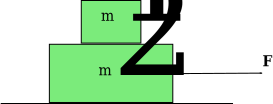
\includegraphics[scale=0.95]{bloques}
    Imagen aqui
  \end{minipage}
  \begin{minipage}{0.6\linewidth}
    \begin{enumerate}
    \item Dibujar todas las fuerzas que actuan sobre cada bloque.
      \label{item:d1a}
    \item Escribir las ecuaciones de movimiento para cada bloque
      \label{item:d1b}
    \item Otra pregunta
      \label{item:d1c}
    \end{enumerate}
  \end{minipage}

  \begin{itemize}
  \item[\ref{item:d1b})] Respuesta 2
  \item[\ref{item:d1c})] Respuesta 3
  \end{itemize}

\newpage

\item Otra pregunta
 
\begin{comentario}
 \item Punto viejo
\end{comentario}

\begin{comentario}
\item Pregunta vieja
\begin{solucion}
    Solucion vieja
\end{solucion}
\end{comentario}

\end{enumerate}
\end{document}
